\begin{figure}[t]
\centering
\definecolor{cVer}{HTML}{0072B2}   % verified (computer-algebra) pairs
\definecolor{cRec}{HTML}{D55E00}   % recipe-family prompts D1-D3
\definecolor{cD4}{HTML}{E69F00}    % D4 restatements (unrelated prompt)
\definecolor{cBT}{HTML}{009E73}    % back-translated positives
\definecolor{cMELD}{HTML}{999999}  % MELD-recipe arm
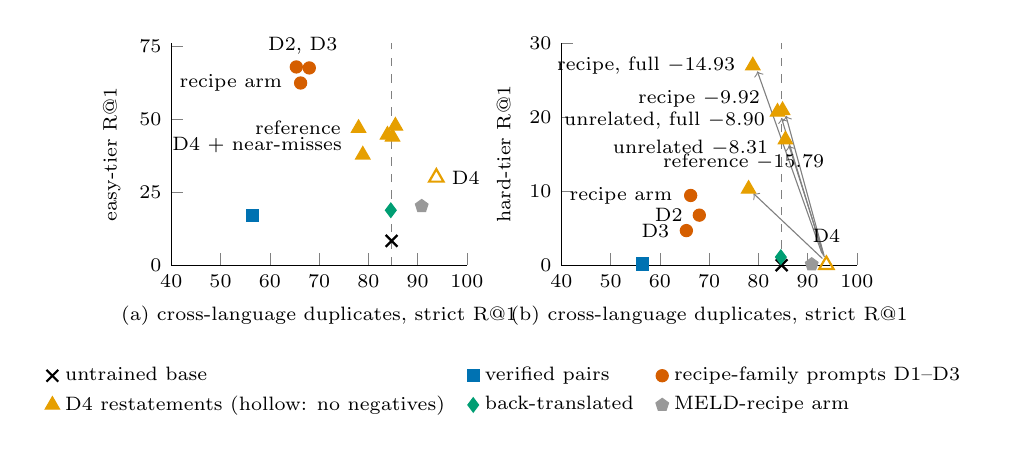
\begin{tikzpicture}
\begin{axis}[
  name=a,
  width=0.44\linewidth, height=4.4cm,
  xmin=40, xmax=100, ymin=0, ymax=76,
  xtick={40,50,60,70,80,90,100}, ytick={0,25,50,75},
  xlabel={(a) cross-language duplicates, strict R@1}, ylabel={easy-tier R@1},
  label style={font=\scriptsize}, tick label style={font=\scriptsize},
  axis y line*=left, axis x line*=bottom, clip=false,
]
\addplot[gray, dashed, forget plot] coordinates {(84.73,0) (84.73,76)};
\addplot[forget plot, only marks, mark=x, mark size=3pt, thick, black] coordinates {(84.73,8.32)};
\addplot[forget plot, only marks, mark=square*, mark size=2.2pt, cVer] coordinates {(56.52,17.05)};
\addplot[forget plot, only marks, mark=*, mark size=2.2pt, cRec] coordinates {(66.26,62.38) (68.02,67.54) (65.39,67.88)};
\addplot[forget plot, only marks, mark=triangle, mark size=3pt, thick, cD4] coordinates {(93.81,30.03)};
\addplot[forget plot, only marks, mark=triangle*, mark size=3pt, cD4] coordinates {(78.02,46.91) (83.89,44.59) (78.88,37.79) (85.50,47.69) (84.91,43.93)};
\addplot[forget plot, only marks, mark=diamond*, mark size=2.6pt, cBT] coordinates {(84.57,18.81)};
\addplot[forget plot, only marks, mark=pentagon*, mark size=2.4pt, cMELD] coordinates {(90.84,20.23)};
\node[font=\scriptsize, anchor=east] at (axis cs:64.5,62.38) {recipe arm};
\node[font=\scriptsize, anchor=south] at (axis cs:66.7,69.0) {D2, D3};
\node[font=\scriptsize, anchor=west] at (axis cs:95.0,30.03) {D4};
\node[font=\scriptsize, anchor=east] at (axis cs:76.4,46.91) {reference};
\node[font=\scriptsize, anchor=east] at (axis cs:76.6,41.2) {D4 + near-misses};
\end{axis}
\begin{axis}[
  name=b, at={(a.south east)}, anchor=south west, xshift=1.2cm,
  width=0.44\linewidth, height=4.4cm,
  xmin=40, xmax=100, ymin=0, ymax=30,
  xtick={40,50,60,70,80,90,100}, ytick={0,10,20,30},
  xlabel={(b) cross-language duplicates, strict R@1}, ylabel={hard-tier R@1},
  label style={font=\scriptsize}, tick label style={font=\scriptsize},
  axis y line*=left, axis x line*=bottom, clip=false,
  legend to name=invlegend, legend columns=3,
  legend style={font=\scriptsize, draw=none, /tikz/every even column/.append style={column sep=6pt}}, legend cell align=left,
]
\addplot[gray, dashed, forget plot] coordinates {(84.73,0) (84.73,30)};
\addplot[only marks, mark=x, mark size=3pt, thick, black] coordinates {(84.73,0.00)};
\addlegendentry{untrained base}
\addplot[only marks, mark=square*, mark size=2.2pt, cVer] coordinates {(56.52,0.16)};
\addlegendentry{verified pairs}
\addplot[only marks, mark=*, mark size=2.2pt, cRec] coordinates {(66.26,9.42) (68.02,6.76) (65.39,4.67)};
\addlegendentry{recipe-family prompts D1--D3}
\addplot[only marks, mark=triangle*, mark size=3pt, cD4] coordinates {(78.02,10.30) (83.89,20.71) (78.88,26.97) (85.50,16.96) (84.91,20.93)};
\addlegendentry{D4 restatements (hollow: no negatives)}
\addplot[forget plot, only marks, mark=triangle, mark size=3pt, thick, cD4] coordinates {(93.81,0.04)};
\addplot[only marks, mark=diamond*, mark size=2.6pt, cBT] coordinates {(84.57,1.09)};
\addlegendentry{back-translated}
\addplot[only marks, mark=pentagon*, mark size=2.4pt, cMELD] coordinates {(90.84,0.11)};
\addlegendentry{MELD-recipe arm}
\draw[->, thin, gray] (axis cs:93.0,0.9) -- (axis cs:79.0,9.7);
\draw[->, thin, gray] (axis cs:93.2,1.3) -- (axis cs:84.7,19.9);
\draw[->, thin, gray] (axis cs:92.9,1.6) -- (axis cs:79.8,26.2);
\draw[->, thin, gray] (axis cs:93.4,1.1) -- (axis cs:86.2,16.2);
\draw[->, thin, gray] (axis cs:93.3,1.4) -- (axis cs:85.6,20.2);
\node[font=\scriptsize, anchor=east] at (axis cs:64.5,9.42) {recipe arm};
\node[font=\scriptsize, anchor=east] at (axis cs:66.6,6.76) {D2};
\node[font=\scriptsize, anchor=east] at (axis cs:63.9,4.67) {D3};
\node[font=\scriptsize, anchor=south] at (axis cs:93.81,1.8) {D4};
\node[font=\scriptsize, anchor=south] at (axis cs:77.0,11.6) {reference $-15.79$};
\node[font=\scriptsize, anchor=east] at (axis cs:77.3,26.97) {recipe, full $-14.93$};
\node[font=\scriptsize, anchor=east] at (axis cs:82.3,22.5) {recipe $-9.92$};
\node[font=\scriptsize, anchor=east] at (axis cs:83.3,19.5) {unrelated, full $-8.90$};
\node[font=\scriptsize, anchor=east] at (axis cs:84.0,15.9) {unrelated $-8.31$};
\end{axis}
\node[anchor=north, yshift=-4pt] at (current bounding box.south) {\pgfplotslegendfromname{invlegend}};
\end{tikzpicture}
\caption{Benchmark score against real retrieval kept after training, one point per trained model. Horizontal axis: strict R@1 on cross-language duplicates; the dashed line and $\times$ mark the untrained base, so points left of it lost real retrieval by being trained. Colour gives the positives (legend); hollow means no negatives. (a)~Easy tier: every model trained on LLM rewrites scores above the verified arm. (b)~Hard tier: only deep LLM rewrites with negatives leave the floor. Arrows run from D4 alone to D4 with negatives attached; each label names the negatives (verified ones give the reference; ``recipe'' and ``unrelated'' are LLM near-misses from the recipe's prompt and from an unrelated one, at the reference's count or at the recipe arm's full volume) and the cross-language points lost. All models: Figure~\ref{fig:inversion-full}.}
\label{fig:inversion}
\end{figure}
\section{What the Recipe Adds, and the Fingerprint It Leaves}
\label{sec:mechanism}

\paragraph{Four rewriter prompts on one ladder, and a factorial over the pair.}
This section uses two designs. The first is a ladder of four prompts. \textbf{D1} is the benchmark's published Appendix-F prompt, near-verbatim, and its model is the recipe arm; \textbf{D2} is a close paraphrase of that prompt; \textbf{D3} asks for the same thing in a clearly different style; \textbf{D4} is a restatement prompt with no connection to the benchmark's. Everything else is held fixed: the same source problems, judge and training settings, and D1 to D3 share one output format, one positive and up to three near-misses, so the ladder changes the wording of the prompt while the shape of each training pair stays the same (Appendix~\ref{app:prompts}); D4 asks for restatements only and writes no negatives. The second design separates D4's prompt from its missing negatives: a grid crossing computer-algebra rewrites or D4 restatements with computer-algebra counterexamples or none, extended with LLM-written near-misses from the recipe's prompt and from an unrelated one and with back-translated positives (Table~\ref{tab:factorial}).


\paragraph{On the hard tier the pair structure scores, both halves are needed, and the recipe-specific part is an increment in the near-misses.}
Before running D2--D4 we predicted that hard-tier R@1 would fall step by step as the prompt moves away from the benchmark's. It did: $9.90 > 6.76 > 4.67 > 0.04$ from D1 to D4, at three seeds per rung and in every seed (Table~\ref{tab:dose-full}). The grid explains the last, large drop. Neither half of a training pair works alone: positives of any kind trained without negatives score $0.00$ to $0.05$. Negatives on shallow positives barely help either: near-copy and back-translated positives stay between $0.11$ and $4.18$ with negatives of any kind (Appendix~\ref{app:mechanism}). The positive has to be a deep LLM rewrite (Section~\ref{sec:limitations}). Give D4's restatements the verified negatives and the result is the reference, at $10.30$ over eight seeds, level with the recipe arm, from a file with no benchmark wording in it; a second recipe-free prompt's restatements with the same negatives reach only $3.97$, so the level a recipe-free file reaches depends on which prompt wrote the restatements. Now change only the negatives, keeping D4's positives (three seeds each; matched to the reference's count, $0.08$ fewer per row): near-misses written under a prompt unrelated to the recipe lift the score to $16.96$ and near-misses written under the benchmark's own prompt to $20.71$; with as many negatives as the recipe arm has, $20.93$ and $26.97$, the last nearly three times the recipe arm (Table~\ref{tab:factorial}). So the tier rewards the recipe's \emph{pair structure}, a deep rewrite against an LLM-written near-miss. Near-misses from either LLM prompt carry most of the step up from verified negatives; the recipe's own add $3.75$ to $6.03$ on top. The template's own positives are not required, and restatements from an unrelated prompt outscore them at either kind of negative: $26.97$ against $9.42$ with the recipe's near-misses, $10.30$ against $2.09$ with verified negatives. One tempting account, that a positive and its near-misses written in one call share phrasing, is ruled out: regenerating the recipe's positives and near-misses in separate calls leaves the tier where it was ($9.79$). Two other accounts are untested (Appendix~\ref{app:mechanism}).

\paragraph{On the easy tier no gradient appears: the genre scores.}We predicted the same step-by-step fall for the easy tier. It does not happen. The only rung that drops is D4, the one with no negatives, and once D4 gets the verified negatives it becomes the reference of Table~\ref{tab:controlled}. D2 and D3 cannot be told apart, their difference flipping sign across seeds, and both score five to six points \emph{above} the recipe arm (Table~\ref{tab:dose-full}), the opposite of the registered direction (Appendix~\ref{app:setup}). The easy tier does not care which LLM prompt wrote the training pairs: any prompt that produces LLM-style rewrites scores, so the tier is gamed at the \emph{genre} level.

\paragraph{The real-data prediction failed: D4 tops cross-language retrieval and every negative that lifts it costs points.}
We had registered that all four rungs would sit just below the base on cross-language duplicates, in a narrow band with no trend; that failed: the rungs spread almost three times wider than the bound and D4 landed above the base (Appendix~\ref{app:mechanism}). D4 sits at the top on cross-language duplicates, $93.81$ against the base's $84.73$, within noise of back-translated positives trained alone ($94.57$; Appendix~\ref{app:mechanism}), at $+0.04$ hard R@1. Every way of giving it negatives buys hard-tier score and pays in cross-language score: the verified negatives that lift it to $10.30$ cost it $15.79$ of those points, the recipe's own near-misses at the reference's count lift it to $20.71$ and cost $9.92$, and near-misses from an unrelated prompt lift it to $16.96$ and cost $8.31$, leaving that model at the base (Figure~\ref{fig:inversion}b). The recipe arm itself, which leads the reference on the easy tier, trails it by $11.77$ on cross-language duplicates (Section~\ref{sec:gaming}; Figure~\ref{fig:inversion}).

\paragraph{An $n$-gram probe finds the LLM fingerprint, and recipe-prompt models track it.}
A plain $n$-gram classifier, trained on our rewrites against their own source problems and tested on sources it never saw, tells LLM rewrites from human-written problems at $0.880$ AUC, detects the benchmark's Gemini-3-flash golds at $0.804$ without having seen a token from that vendor, and separates the benchmark's golds from its own near-misses at $0.750$ with no retriever involved, so a style difference between right and wrong answers is built into its pairs; the recipe-free D4 rewrites are detected at $0.676$ and D1--D3 somewhat more strongly, and that climb is what the recipe adds (Table~\ref{tab:panel}). Correlating each model's similarities with that style score across documents, query by query, shows neither the base nor the verified arm tracking style; the recipe arm does ($\rho = +0.171$, above the verified arm on $94.2\%$ of queries), D2 and D3 do too, D4 does not, and the reference and the D4 cells trained with the recipe's near-misses show only a trace ($+0.025$ to $+0.050$). The habit comes from the recipe's rewrite prompts as a family, not the template alone, and the cells that buy the most hard-tier score carry little of it: chasing style is not what buys the tier (Table~\ref{tab:style}). The $1{,}401$ hard-tier queries the recipe arm alone wins skew toward golds sharing the query's wording, not toward LLM-styled golds (Section~\ref{sec:limitations}).
